% ### Uses XeLaTeX ### %
% ### Needs beamer-master ### %
\documentclass[aspectratio=169]{beamer} %. Aspect Ratio 16:9
\usetheme{AI2} % beamerthemeSprace.sty
% DATA FOR FOOTER
\date{2020}
\title{}
\author{}
\institute{Advanced Institute for Artificial Intelligence (AI2)}
\begin{document}    
% ####################################
% FIRST SLIDE 						:: \SliTit{<Title of the Talk>}{<Author Name>}{<Intitution>}
% SLIDE SUB-TITLE					:: \SliSubTit{<Title of the Chapter>}{<Title of the Section>}
% SLIDE WITH TITLE 					:: \SliT{<Title>}{Content}
% SLIDE NO TITLE 						:: \Sli{<Content>} 
% SLIDE DOUBLE COLUMN WITH TITLE 	:: \SliDT{<Title>}{<First Column>}{<Second Column>}
% SLIDE DOUBLE COLUMN NO TITLE 		:: \SliD{<First Column>}{<Second Column>}
% SLIDE ADVANCED WITH TITLE 			:: \SliAdvT{<Title>}{<Content>}
% SLIDE ADVANCED  NO TITLE 			:: \SliAdv{<Content>}
% SLIDE ADVANCED DOUBLE TITLE 		:: SliAdvDT{<Title>}{<First Column>}{<Second Column>}
% SLIDE ADVANCED DOUBLE NO TITLE 	:: SliAdvD{<First Column>}{<Second Column>}
% ITEMIZE 							:: \begin{itemize}  \IteOne{1st Level} \IteTwo {2nd Level} \IteThr{3rd Level} \end{itemize}
% SECTION 							:: \secx{Section} | \secxx{Sub-Section}
% COLOR BOX 						:: \blu{blue} + \red{red} + \yel{yellow} + \gre{green}
% FRAME 							:: \fra{sprace} \frab{blue} \frar{red} + \fray{yellow} + \frag{green}	
% REFERENCE						:: \refer{<doi number>}
% FIGURE 							::  \img{X}{Y}{<scale>}{Figures/.png} 
% FIGURE							:: \begin{center}\includegraphics[scale=<#>]{Figures/.png}\end{center}
% PROJECT STATUS					:: \planned\~    \started\~   \underway\~   \done\~   
% EXERCICIO							:: \Exe{<#>}{<text>}
% STACKREL							:: \underset{<down>}{<up>}
% FLUSH LEFT						:: \begin{flalign*}  & <1st equation> & \\  & <12nd equation>  & \\ \end{flalign*}
% REAL / IMAGINAY					:: \Re / \Im
% SLASH								:: \sl{} or \sl
% BOLD MATH							:: \pmb{<>}
% ####################################
%
% FIRST SLIDE :: DO NOT BREAK LINE !!!
\SliTit{Python}{Advanced Institute for Artificial Intelligence}{https://advancedinstitute.ai}

% SLIDE WITH TITLE
\SliT{Sumario}{

\begin{itemize}
  \IteOne{Introdução}
  \IteOne{Estruturas e Função de Controle}
  \IteOne{Coleções}
  \IteOne{Programação Orientada a Objetos}
  \IteOne{Manipulação de arquivos}
  \IteOne{Processos e Threading}  
\end{itemize}

}

% SLIDE WITH TITLE
\SliT{Introdução}{

\secx{Python}

\begin{itemize}
    \IteOne{Python é uma linguagem interpretada}
\end{itemize}
\secxx{Interpretada x Compilada}

\begin{itemize}
    \IteOne{\textbf{Interpretada}: Python, Perl, Lua}
    \IteOne{\textbf{Compilada}: C, Fortran, C#}
\end{itemize}
}
\Sli{
\begin{itemize}
    \IteOne{Criada nos anos 90, se tornou extremamente popular nos últimos anos.}
\end{itemize}

\begin{figure}
    \centering
    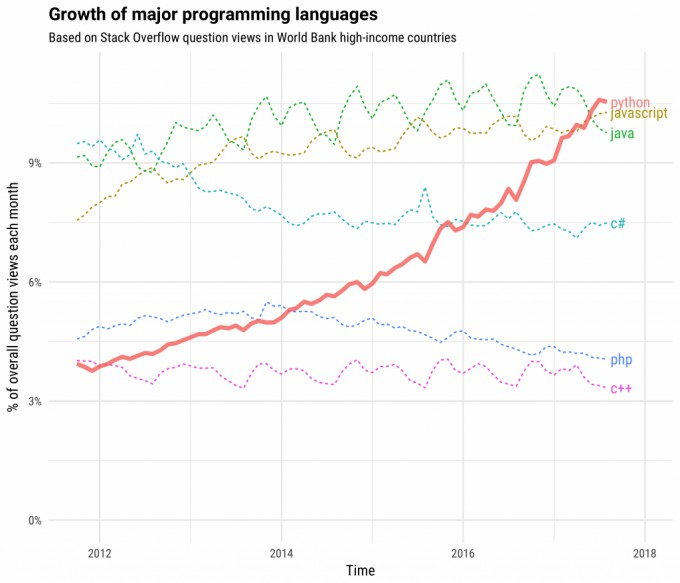
\includegraphics[scale=0.32]{growthpython.jpg}
    
    \label{fig:my_label}
\end{figure}

}

\Sli{
\begin{figure}
    \centering
    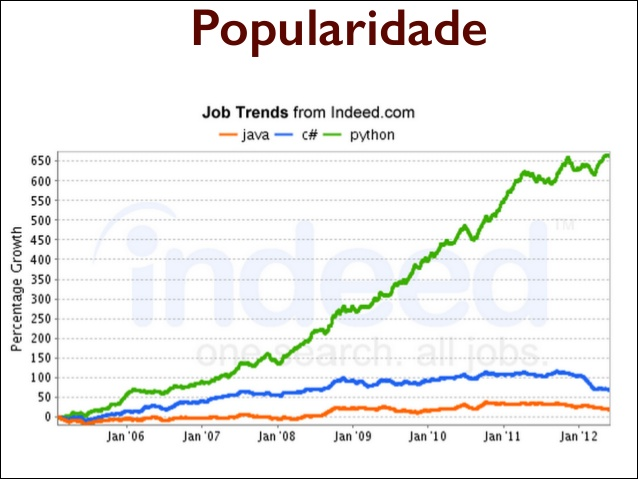
\includegraphics[scale=0.4]{growthpython2.jpg}
    \label{fig:my_label}
\end{figure}
}



\begin{SliTC}{Introdução}
   \begin{itemize}

  \IteOne{Caminho do Python no Sistema}
  \end{itemize}
  \begin{lstlisting}[language=python]
which python
   \end{lstlisting}
   \begin{itemize}
      \IteOne{Versão do Python} 
   \end{itemize}
  \begin{lstlisting}[language=python]
python -V
   \end{lstlisting}
\end{SliTC}






% SLIDE WITH TITLE
\begin{SliTC}{Usando Python}

\begin{itemize}
  \IteOne{Iniciando interpretador Python}
  \begin{lstlisting}[language=python]
python
   \end{lstlisting}
   \IteTwo{Python 3.6.8 |Anaconda, Inc.| (default, Dec 30 2018, 01:22:34) }
  \IteTwo{[GCC 7.3.0] on linux}
  \IteTwo{Type "help", "copyright", "credits" or "license" for more information.}
  \IteTwo{$>>>$ Esse é o prompt para receber comandos python }
  \IteOne{Ctrl+D sai do interpretador }
\end{itemize}
\end{SliTC}


\Sli{
\begin{itemize}
    \IteOne{O Python tem duas versões principais: 2 e 3}
    \IteOne{Sempre que possível deve-se utilizar Python 3}
    \IteOne{Entretando, alguns códigos e bibliotecas só são compatíveis com Python 2, portanto pode ser que tenhamos que utilizá-lo algumas vezes.}
\end{itemize}


}

% SLIDE WITH TITLE
\begin{SliTC}{Usando Python}

\secxx{Comando print}

\begin{itemize}
  \IteOne{Python 2}
  \begin{lstlisting}[language=python]
print "hello world"
   \end{lstlisting}
\IteOne{Python 3}
  \begin{lstlisting}[language=python]
print ("hello world")
   \end{lstlisting}
  \IteOne{print "hello world"}
\end{itemize}

\secxx{Comentários no código}
\begin{itemize}
  \IteOne{\# : comentando uma linha}
  \IteOne{''' : começar e terminar bloco de comentário}
  \IteOne{""" : começar e terminar bloco de comentário}
\end{itemize}

\end{SliTC}

% SLIDE WITH TITLE
\begin{SliTC}{Usando Python}

\secxx{Indentação}

\begin{itemize}
  \IteOne{O controle de início e fim de blocos de código é feito por meio de Indentação}
  \IteOne{Indentação pode ser controlada por um tamanho fixo de espaços em branco}
  \IteOne{Exemplo}
  \begin{lstlisting}[language=python]
print ("teste")
if (i == 0):
    print ("0")
else:
    print ("outro valor")
    if (i >= 0):
        print (">=0")
   \end{lstlisting}

\end{itemize}


\end{SliTC}
% SLIDE WITH TITLE
\SliT{Tipos de dados - Números}{

Existem três tipos numéricos em python: números inteiros, números de ponto flutuante e números complexos. 

\begin{itemize}
  \IteOne{Booleanos são um subtipo de números inteiros. }
  \IteOne{Inteiros têm precisão ilimitada.}
  \IteOne{Números de ponto flutuante são geralmente implementados usando tipo Double em C}
\end{itemize}

}

\begin{SliTC}{Operações com Números}

\begin{itemize}
    \IteOne{$=$: Sempre usado para \textbf{atribuições}}
    \IteOne{$==$, $!=$, $<>$, $>$, $<$, $>=$, $<=$: Comparações}
\end{itemize}

\begin{lstlisting}[language=python]
a = 10
b = 5
print(a == b)
print(a != b)
print(a <> b)
print(a > b)
print(a < b)
print(a >= b)
print(a <= b)
\end{lstlisting}

\end{SliTC}

\SliT{Tipos de dados - Strings}{

Strings podem ser manipuladas de diversas maneiras em Python

\begin{itemize}
  \IteOne{podem ser representadas usando aspas simples ' ' ou aspas duplas " "  }
  \IteOne{É possível utilizar catacteres escape   }

\end{itemize}

}


\SliT{Funções}{

\begin{itemize}
  \IteOne{A palavra-chave def é usada para definir funções}
  \IteOne{Deve ser definida antes de ser utilizada}
  \IteOne{O valor de retorno padrão é None}
\end{itemize}

}

\SliT{Função}{
Argumento pode ser gerado da seguinte forma:
\begin{enumerate}
  \IteOne{nome de variável}
  \IteOne{nome de variável e valor padrão}
\end{enumerate}

Escopo de variável
\begin{itemize}
  \IteOne{variáveis possuem escopo local ao bloco onde são criadas}
  \IteOne{Pode ser definidas variáveis globais}
\end{itemize}

}

\begin{SliTC}{Funções}
\secxx{Função sem argumentos}:
\begin{lstlisting}[language=python]
def greeting():
    print("hello world")

greeting()
\end{lstlisting}
\end{SliTC}

\begin{SliTC}{Argumento de Função}
\begin{lstlisting}[language=python]
def numsquare(num):
    return num * num

number=10

numsquare(number)

def numsquare(num=10):
    return num * num

numsquare()
\end{lstlisting}

\end{SliTC}

\begin{SliTC}{Obtendo dados do usuário}

\secxx{A função input() é utilizada para aguardar um valor digitado no terminal pelo usuário}
\begin{lstlisting}[language=python]
usrip = input("numero inteiro: ")
usrnum = int(usrip)
sqrnum = numsquare(usrnum)
print("O quadrado do numero eh: {}".format(sqrnum))

usrip = input("float: ")
usrnum = float(usrip)
sqrnum = numsquare(usrnum)
print("O quadrado do numero eh: {}".format(sqrnum))

usrname = input("nome: ")
print("nome: ",usrname)
\end{lstlisting}

\end{SliTC}

\begin{SliTC}{Usando bibliotecas adicionais}

\secxx{A palavra reservada {\color{red}import} permite adicionar pacotes que não são nativos do Python}

\begin{lstlisting}[language=python]
import subprocess

# Executa um comando linux no terminal

subprocess.call('date')
\end{lstlisting}
A palavra reservada {\color{red}from} permite importar apenas parte de um pacote 
\begin{lstlisting}[language=python]
from sklearn.model_selection import train_test_split
\end{lstlisting}

\end{SliTC}

\SliT{Estruturas e Função de Controle}{

\secxx{As funções padrão de controle de fluxo de execução estão disponíveis no Python:}
\begin{itemize}
  \IteOne{if}
  \IteOne{for}
  \IteOne{while}
\end{itemize}

}

\begin{SliTC}{Estruturas e Função de Controle}

\secx{if} 
\begin{itemize}
  \IteOne{As instruções if avaliam uma condição, caso seja verdadeira executa o bloco seguinte}
  \IteOne{Pode ser combinado com uma estrutura else, que é executada quando a condição não é verdadeira no bloco if}
\end{itemize}

Exemplo:

\begin{lstlisting}[language=python]
var = 100

if (var==100):
    print("100")
else: 
    print("not 100")
\end{lstlisting}
\end{SliTC}

\begin{SliTC}{Estruturas e Função de Controle}

\secxx{for}
\begin{itemize}
    \IteOne{executam um certo bloco de código para um número conhecido de iterações. }
    \IteOne{Um bloco de código pode ser executado para o número de itens existentes em uma lista, dicionário, variável de sequência ou tupla}
    \IteOne{Um bloco de código pode ser executado em um intervalo contado de etapas}
\end{itemize}

\secxx{Exemplo}

\begin{lstlisting}[language=python]
a=(10,20,30,40,50)
for b in a:
    print ("square of " + str(b) + " is " +str(b*b))
\end{lstlisting}
\end{SliTC}

\begin{SliTC}{Estruturas e Função de Controle}

\secxx{while}

\begin{itemize}
    \IteOne{O loop while é executado enquanto uma declaração condicional retorna true }
    \IteOne{A instrução condicional é avaliada toda vez que um bloco de código é executado }
    \IteOne{A execução para no momento em que a instrução condicional retorna false. }
\end{itemize}

Exemplo:

\begin{lstlisting}[language=python]
count = 0
while (count $<$ 9):
    print("iteração",count)
    count+=1
\end{lstlisting}

\end{SliTC}

\begin{SliTC}{Operadores Lógicos}
\secxx{Principais Operadores Lógicos}
\begin{itemize}
    \IteOne{\textit{and}}
    \IteOne{\textit{or}}
    \IteOne{\textit{not}}
\end{itemize}
\begin{lstlisting}[language=python]
x = True
y = False

print('x and y is',x and y)
print('x or y is',x or y)
print('not x is',not x)
\end{lstlisting}
x and y is False \\
x or y is True \\
not x is False 
\end{SliTC}

\begin{SliTC}{Coleções}

\begin{itemize}
    \IteOne{Coleções são implementações de estrutura de dados} 
    \IteOne{Permitem guardar e manipular conjuntos de valores de maneira organizada e otimizada}
\end{itemize}
\begin{lstlisting}[language=python]
friends = [ 'Joseph', 'Glenn', 'Sally' ]
carryon = [ 'socks', 'shirt', 'perfume' ]
\end{lstlisting}
\end{SliTC}

\Sli{
\secx{Coleções em python:}
\begin{itemize}
    \IteOne{list}: Lista
    \IteOne{set}: Conjunto
    \IteOne{dictionary}: Dicionárop / Hash Table
    \IteOne{tuple}: Tupla
    \IteOne{entre outros....}
\end{itemize}
}

\SliDT{List}{

Os elementos na lista (list) são separados por vírgulas.

Um elemento da lista pode ser qualquer objeto Python - até outra lista

Uma lista pode estar vazia

Operador index representa uma posição na lista
}{
list = [1, 24, 76]

list = ['red', 'yellow', 'blue']

list = ['red', 24, 98.599999999999994]

list = [1, [5, 6], 7]

l[0] =$>$ 1
}

\begin{SliTC}{List}

\begin{itemize}
    \IteOne{Listas são mutáveis} 
\end{itemize}
\begin{lstlisting}[language=python]
lotto = [2, 14, 26, 41, 63]
print(lotto)
\end{lstlisting}
[2, 14, 26, 41, 63]

\begin{lstlisting}[language=python]
lotto[2] = 28
print(lotto)
\end{lstlisting}
[2, 14, 28, 41, 63]

\begin{itemize}
    \IteOne{Operador \textbf{len} retorna tamanho da lista} 
\end{itemize}

\begin{lstlisting}[language=python]
print (len(lotto))
\end{lstlisting}
5
\end{SliTC}


\SliT{List}{
\secx{Operaçòes}
\begin{itemize}
    \IteOne{\textbf{append}: Adiciona elementos no fim da lista}
    \IteOne{\textbf{in}: pode ser usado para verificar se um elemento existe na lista}
    \IteOne{\textbf{sort}: Ordena a lista}
    \IteOne{\textbf{split}: Quebra uma string em partes menores usando estrutura de lista}
\end{itemize}
}

\SliT{Dicionários}{

\secx{Dicionários são uma implementação de hashtable}
\begin{itemize}
    \IteOne{Mapeia "chaves" para valores}
\end{itemize}

\secxx{Operações:} 
\begin{itemize}
    \IteOne{print, del, len, in} 
\end{itemize}
\secxx{Métodos: } 
\begin{itemize}
    \IteOne{keys(), values(), items()} 
\end{itemize}
}

\begin{SliTC}{Dicionários}

\begin{lstlisting}[language=python]
eng2sp = {}
eng2sp['one'] = 'uno'
eng2sp['two'] = 'dos'

eng2sp = { 'one': 'uno', 'two': 'dos', 'three':'tres' }
\end{lstlisting}


\end{SliTC}
%Aqui


\begin{SliTC}{List Comprehensions}

\secxx{Aplica uma expressão a cada elemento da lista}

\begin{lstlisting}[language=python]
vec = [2, 4, 6]
[3*x for x in vec]
\end{lstlisting}
[6, 12, 18]

\begin{lstlisting}[language=python]
 [3*x for x in vec if x > 3]
\end{lstlisting}
 [12, 18]
\end{SliTC}

\begin{comment}
\SliT{Tupla}{

uma sequência ordenada de elementos, pode misturar tipos de elementos
não pode alterar os valores dos elementos (imutável)

}
\end{comment}

\begin{SliTC}{Slicing}

\begin{itemize}
    \IteOne{Listas podem ser filtradas por meio de 'slicing'} 
    \IteOne{Formato para realizar 'slicing' em uma lista:}
\end{itemize}
\begin{lstlisting}[language=python]
 s[start:end:step]
\end{lstlisting}
\secxx{Elementos:}

\begin{itemize}
    \IteOne{\textbf{s}: um objeto que pode ser manipulado por 'slicing' }
    \IteOne{\textbf{start}: primeiro índice para iniciar a iteração }
    \IteOne{\textbf{end}: último indíce, NOTE que o índice final não será incluído na fatia resultante }
    \IteOne{\textbf{step}: escolha o elemento a cada índice de etapa }
\end{itemize}


\end{SliTC}

\begin{SliTC}{Slicing}{

\secxx{Alguns Exemplos:}

\begin{itemize}
    \IteOne{Selecionar itens a partir do índice start até stop-1 }
\end{itemize}
\begin{lstlisting}[language=python]
 a[start:stop] 
\end{lstlisting}
\begin{itemize}
    \IteOne{Selecionar itens a partir do índice start até o final }
\end{itemize}

\begin{lstlisting}[language=python]
 a[start:] 
\end{lstlisting}
\begin{itemize}
\IteOne{Selecionar itens a partir do início start até stop-1 }
\end{itemize}

\begin{lstlisting}[language=python]
 a[:stop] 
\end{lstlisting}
    
\begin{itemize}
\IteOne{Selecionar itens a partir do início até o final }
\end{itemize}

\begin{lstlisting}[language=python]
 a[:]  
\end{lstlisting}
\end{SliTC}

\begin{SliTC}{Slicing}{

\secxx{Alguns Exemplos:}

\begin{itemize}
    \IteOne{Selecionar itens a partir do índice start não passando de stop-1, realizando pulos definidos na variável step}
\end{itemize}
\begin{lstlisting}[language=python]
 a[start:stop:step] 
\end{lstlisting}
\begin{itemize}
    \IteOne{Último item da lista}
\end{itemize}
\begin{lstlisting}[language=python]
 a[-1] 
\end{lstlisting}
\begin{itemize}
    \IteOne{Últimos dois itens da lista}
\end{itemize}
\begin{lstlisting}[language=python]
 a[-2:]
\end{lstlisting}
\begin{itemize}
    \IteOne{Tudo menos os dois últimos}}
\end{itemize}
\begin{lstlisting}[language=python]
 a[:-2]
\end{lstlisting}
\end{SliTC}

\begin{SliTC}{Slicing}

\secxx{Alguns Exemplos:}

\begin{itemize}
    \IteOne{Quando a lista possuir mais de uma dimensão, é necessário realizar o slicing separadamente em cada dimensão}
\end{itemize}

\begin{itemize}
    \IteOne{Apagando elementos de uma lista}
\end{itemize}
\begin{lstlisting}[language=python]
 del a[3:7] 
\end{lstlisting}
\end{SliTC}
%Aqui
\begin{SliTC}{Manipulação de Texto}

\secxx{Abrir um arquivo:}

\begin{itemize}
    \IteOne{Preparar o arquivo para leitura:}
    \IteOne{Vincula a variável do arquivo ao arquivo físico} 
    \IteOne{Posiciona o ponteiro do arquivo no início do arquivo.} 
\end{itemize}

Formato:
\begin{lstlisting}[language=python]
 <variável do arquivo> = open (<nome do arquivo>, "r")
\end{lstlisting}
     

Exemplo:

\begin{lstlisting}[language=python]
inputFile = open ("data.txt", "r")
    
filename = input ("Digite o nome do arquivo de entrada:")
    
inputFile = open (filename, "r")
\end{lstlisting}
    
\end{SliTC}

\begin{SliTC}{Manipulação de Texto}

\secxx{Comando para fechar um arquivo}
Formato:
\begin{lstlisting}[language=python]
<name of file variable>.close()
\end{lstlisting}
Exemplo:

\begin{lstlisting}[language=python]
inputFile.close()
\end{lstlisting}

\end{SliTC}

\begin{SliTC}
{Manipulação de Texto}
\begin{itemize}
    \IteOne{Normalmente, a leitura é feita dentro do corpo de um loop}
    \IteOne{Cada execução do loop lê uma linha do arquivo em uma string}
\end{itemize}
\begin{lstlisting}[language=python]
for <variavel para armazenar uma sequencia> em <nome da variavel do arquivo>:

    <Faca algo com a string lida no arquivo>

\end{lstlisting}
Exemplo:

\begin{lstlisting}[language=python]
for line in inputFile:
    print (line) 
\end{lstlisting}
\end{SliTC}


%\SliT{Manipulação de Texto}{

%Escrita de arquivo

%Exemplo 1:

%f = open("f.txt", "w")

%f.write("teste")

%f.close()    

%Exemplo 2:

%with open("new_file.txt", "w") as f:

%    f.write("This is a sample line of text\n")
    
%    f.write("Yet another line\n")

%}
\SliTit{Programação Orientada a Objetos}{Advanced Institute for Artificial Intelligence}{https://advancedinstitute.ai}

\SliT{Orientação a objeto}{

\secxx{Orientação a Objetos surgiu da necessidade de modelar sistemas complexos}

\begin{itemize}
    \IteOne{Modelar problemas utilizando um conjunto de componentes autocontidos, e integráveis}
    \IteOne{Determinar como um objeto deve se comportar e como deve interagir com outros objetos}
\end{itemize}

Algumas iniciativas:

\begin{itemize}
    \IteOne{Simula 67 (60)}
    \IteOne{Smalltalk (70)}
    \IteOne{C++ (80)}
\end{itemize}

}



\SliT{Orientação a objeto}{

\secxx{Conceitos essenciais:}
\begin{itemize}
    \IteOne{Classes e objetos}
    \IteOne{Atributos e Métodos}
    \IteOne{Herança}
    \IteOne{Encapsulamento}
\end{itemize}

}

\SliT{Orientação a objeto}{

Os objetos reais possuem duas caracterísicas:

\begin{itemize}
    \IteOne{Atributos (Estado)}
    \IteOne{Comportamento}
\end{itemize}

Exemplos:
\begin{itemize}
    \IteOne{cachorro}
    \IteTwo{Atributos: nome, cor, raça}
    \IteTwo{Comportamento: latindo, abanando o rabo, comendo}
\end{itemize}

}

\SliT{Orientação a objeto}{

\secxx{Um objeto de software é conceitualmente similar aos objetos reais}

\begin{itemize}
    \IteOne{Objetos armazenam seu estado em atributos}
    \IteTwo{Correspondentes às variáveis em programação estruturada.}

    \IteOne{Objetos expõem seu comportamento através de métodos}
    \IteTwo{Correspondentes às funções em programação estruturada.}
\end{itemize}

}


\SliT{Orientação a objeto}{

\secxx{Exemplos de objeto:}

\begin{itemize}
    \IteOne{Gerenciador de Dados de Alunos}
    \IteTwo{Atributos: lista de alunos}
    \IteTwo{Comportamentos: filtrar alunos por nome, incluir aluno, alterar aluno}
\end{itemize}

\begin{itemize}
    \IteOne{Biblioteca Matemática}
    \IteTwo{Atributos: Matriz }
    \IteTwo{Comportamentos: calcular transposta, multiplicar, somar }
\end{itemize}

}

\SliT{Orientação a objeto}{

\secxx{Empacotar o código em objetos individuais fornece:}
\begin{itemize}
    \IteOne{Modularidade }
    \IteTwo{Objetos são independente}
    \IteOne{Encapsulamento }
    \IteTwo{Os detalhes da implementação de um objeto permanecem ocultos}
    \IteOne{Reuso }
    \IteTwo{Objetos podem ser reutilizados em diferentes programas}
    \IteOne{Fraco acoplamento }
    \IteTwo{Objetos podem ser substituídos facilmente}
\end{itemize}

}

\SliT{Orientação a objeto}{

Uma classe é o projeto a partir do qual objetos individuais são criados

\begin{itemize}
    \IteOne{Ela define os atributos e os métodos correspondentes aos seus objetos. }
    \IteOne{Outros possíveis membros de uma classe são:}
    \IteTwo{Construtores: define as operações a serem realizadas quando um objeto é instanciado.}
    \IteTwo{Destrutores: define as operações a serem realizadas quando um objeto é destruído.}
\end{itemize}

}

\SliT{Orientação a objeto}{

Outras características de uma classe:

\begin{itemize}
    \IteOne{Uma classe pode herdar características de outra classe e incluir novas características}
    \IteOne{Atributos de uma classe podem ser protegidos, sendo possível alterar seu conteúdo por meio apenas de métodos da própria classe}
    \IteOne{Métodos podem ser reescritos}
\end{itemize}

}

\SliT{Orientação a objeto}{

\begin{itemize}
    \IteOne{O relacionamento de Herança define um relacionamento do tipo generalização}
    \IteOne{Indica que uma classe (subclasse) é especializada para gerar uma nova (superclasse)}
    \IteOne{Tudo que a superclasse possui, a subclasse também vai possuir}
    \IteOne{Em Python, todas as classes herdam a classe Object}
\end{itemize}

}


\begin{frame}[fragile] \frametitle{Orientação a objeto}

\begin{center}
    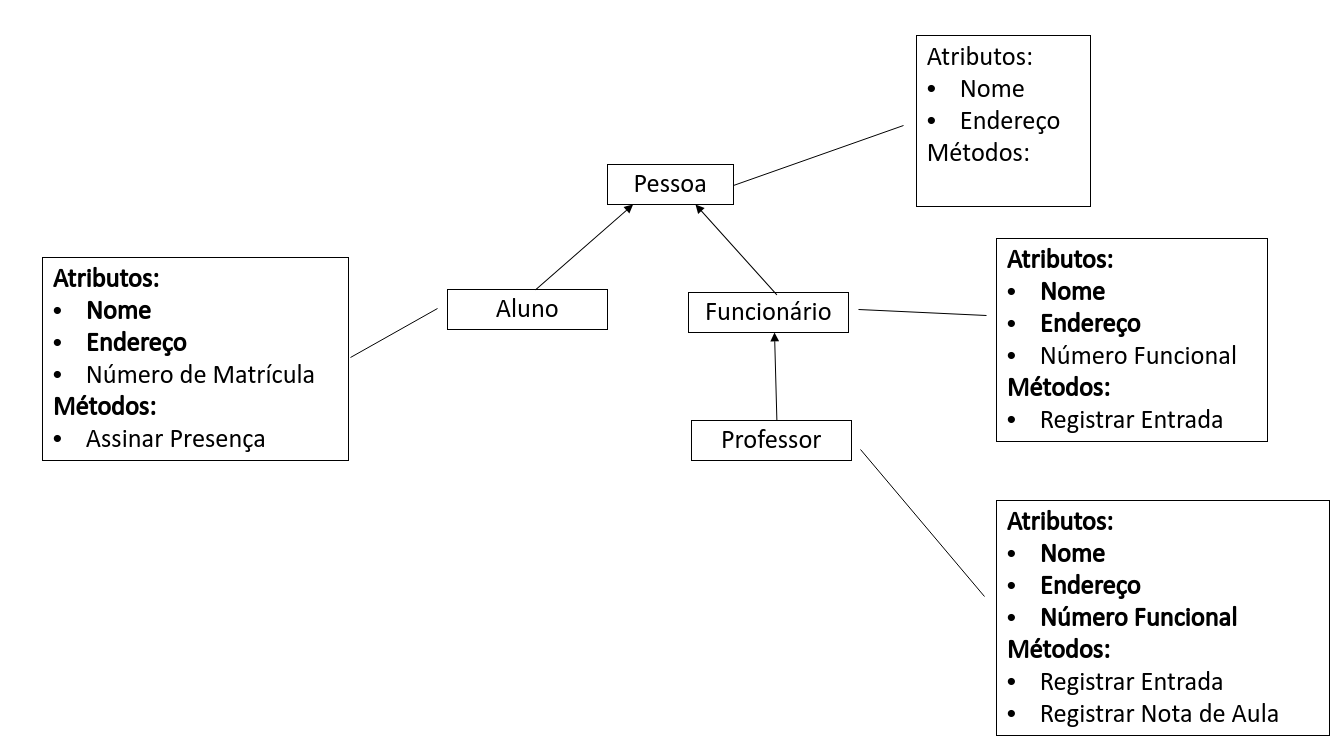
\includegraphics[scale=0.27]{heranca1.png}     
    \end{center}
}

\end{frame}

\begin{SliTC}

 \frametitle{Orientação a objeto}
\secxx{Método Construtor em Python}

\begin{lstlisting}[language=python]
def __init__(self):
    Comandos do construtor
\end{lstlisting}

    

\secxx{Parâmetro para referenciar ao objeto criado: {\color{red}self}}

\begin{itemize}
    \IteOne{Para acessar e criar atributos em um objeto, o caracter "." deve ser usado após o nome do objeto.}
\end{itemize}

\begin{lstlisting}[language=python]
class Critter:
    def __init__(self, name):
        self.name = name
\end{lstlisting}
\end{SliTC}

\begin{SliTC}{Orientação a objeto}

\secxx{A Convenção para definir Métodos ou variáveis privados em Python é colocar como prefixo de seu nome "\_\_"}

PS: Não existem elementos privados "verdadeiros" em Python. É possível acessar qualquer método/atributo de uma classe.

\begin{itemize}
    \item Exemplo:
\end{itemize}
\begin{lstlisting}[language=python]
__a 
__my_variable
\end{lstlisting}

\secxx{Heranças são definidas na declaração da classe, logo após seu nome}

\begin{lstlisting}[language=python]
class teste(object):
    def __init__(self, X):
        self.X = X
\end{lstlisting}
\end{SliTC}

\begin{SliTC}{Orientação a objeto}

\secxx{Exemplo de uma classe em Python}
\begin{lstlisting}[language=python]
class MyClass:
    def function(self):
        print("This is a message inside the class.")
\end{lstlisting}
\secxx{Instanciando um objeto e chamando métodos:}
\begin{lstlisting}[language=python]
myobjectx = MyClass()
myobjectx.function()
\end{lstlisting}

\end{SliTC}


\begin{SliTC}{Orientação a objeto}

\secxx{Exemplo de uma classe em Python}
\begin{lstlisting}[language=python]
# Classe que representa uma coordenada X Y
class Coordinate(object):
    #define um construtor
    def __init__(self, x, y):
        # configura coordenada x e y
        self.x = x
        self.y = y
    #reimplementa a função __str__    
    def __str__(self):
        # Representação em string da coordenada
        return "<" + str(self.x) + "," + str(self.y) + ">"
\end{lstlisting}
\end{SliTC}

\begin{SliTC}{Orientação a objeto}

\begin{lstlisting}[language=python]
def distance(self, other):
    # Calcula distancia euclidiana entre dois pontos
    x_diff_sq = (self.x-other.x)**2
    y_diff_sq = (self.y-other.y)**2
    return (x_diff_sq + y_diff_sq)**0.5
\end{lstlisting}

\secxx{Teste de Uso da Classe}
\begin{lstlisting}[language=python]
c = Coordinate(3,4)
origin = Coordinate(0,0)
print("Coordenada 1:")
print(c)
print(c.distance(origin))
\end{lstlisting}
\end{SliTC}

\begin{SliTC}{Orientação a objeto}
\secxx{Teste com atributos protegidos}

\begin{lstlisting}[language=python]
class MyClass:
    __variable = 0
    def setvariable(self,newvar):
        self.__variable = newvar
    def getvariable(self):
        return (self.__variable)
    def function(self):
        print("This is a message inside the class.")
\end{lstlisting}
\end{SliTC} 



\begin{SliTC}{Orientação a objeto}
\secxx{Teste com atributos protegidos}

\begin{lstlisting}[language=python]
var="rs2"
myobjectx = MyClass()
myobjectx.function()
print(myobjectx.getvariable())
var="rs3"
myobjectx.setvariable(var)
print(myobjectx.getvariable())
\end{lstlisting}
\end{SliTC}

\SliT{Criando Pacotes para Compartilhamento de Classes}{

}

\SliT{MultiThreading}{

}

\end{frame}

\end{document}